\section{Validaci\'on}

La verificaci\'on del modelo propuesto comienza con la simulaci\'on num\'erica de los problemas utilizados hasta esta etapa. Por un lado, se llev\'o a cabo la resoluci\'on del problema de construcci\'on de Maxwell en una cavidad c\'ubica, destinada a verificar el tratamiento de la inconsistencia termodin\'amica por parte del modelo de Xu. Por otro lado, se verific\'o la capacidad de la \lbe{} propuesta para reproducir adecuadamente la transferencia de calor en un fluido van der Waals estratificado y en el avance de un frente de evaporaci\'on.



\subsection{Construcci\'on de Maxwell} 

La base de un problema de construcci\'on de Maxwell es similar a la utilizada en el \chap{chap:isot}, y consiste en simular la evoluci\'on de un fluido en condiciones de saturaci\'on dentro de una cavidad peri\'odica, comparando las densidades reproducidas dentro de cada fase con aquellas determinadas por la ecuaci\'on de estado utilizada. En este caso, el dominio simulado consiste en una cavidad c\'ubica de $100 \times 100 \times 100$ unidades de grilla, con condiciones de contorno peri\'odicas, temperatura uniforme, sin fuerzas externas, y que inicialmente contiene un fluido con densidad perturbada aleatoriamente en  $\pm 1\%$ alrededor del valor cr\'itico ($\rho=\rho_c$). Como se ejemplifica en la \fig{fig:maxwell_3d}, en los primeros instantes comienzan a generarse regiones de diferente densidad, que contin\'uan separ\'andose y agrup\'andose hasta formar estructuras con densidades claramente diferentes. De esta manera, pueden tomarse los valores de densidad en el interior de cada fase, lejos de las interfases, y compararlos con los determinados por la regla de Maxwell.

\begin{figure}[htb]
    \centering
    \begin{subfigure}[t]{0.45\textwidth}
        \centering
        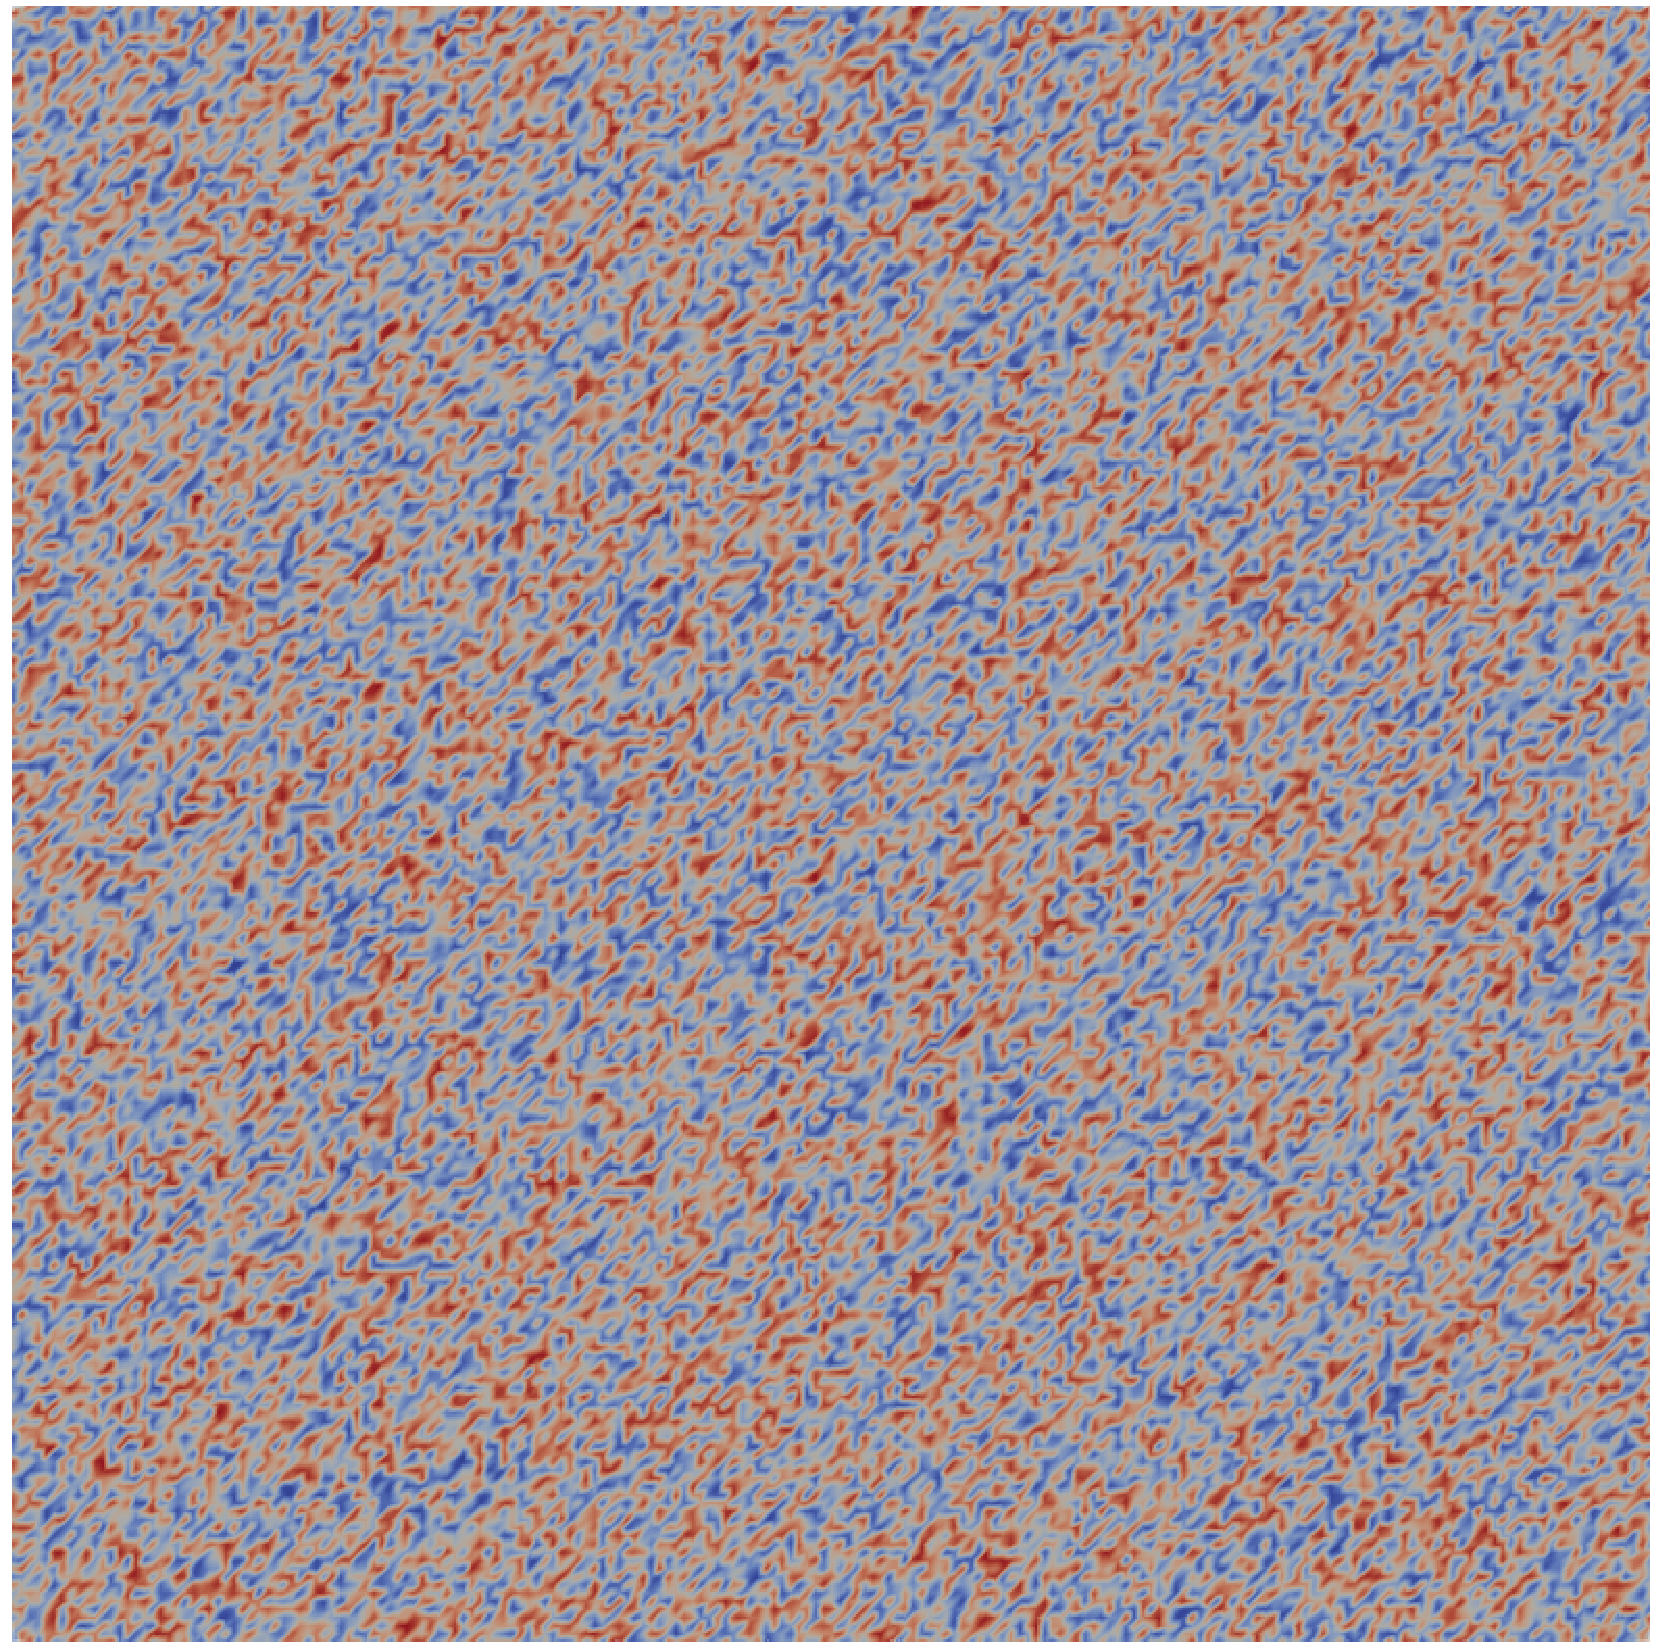
\includegraphics[width=0.95\textwidth]{Imagenes/Maxwell2D/Maxwell2D_sim/Imagenes/t_0}
        \caption{$t=0$}
    \end{subfigure}
    \begin{subfigure}[t]{0.45\textwidth}
        \centering
        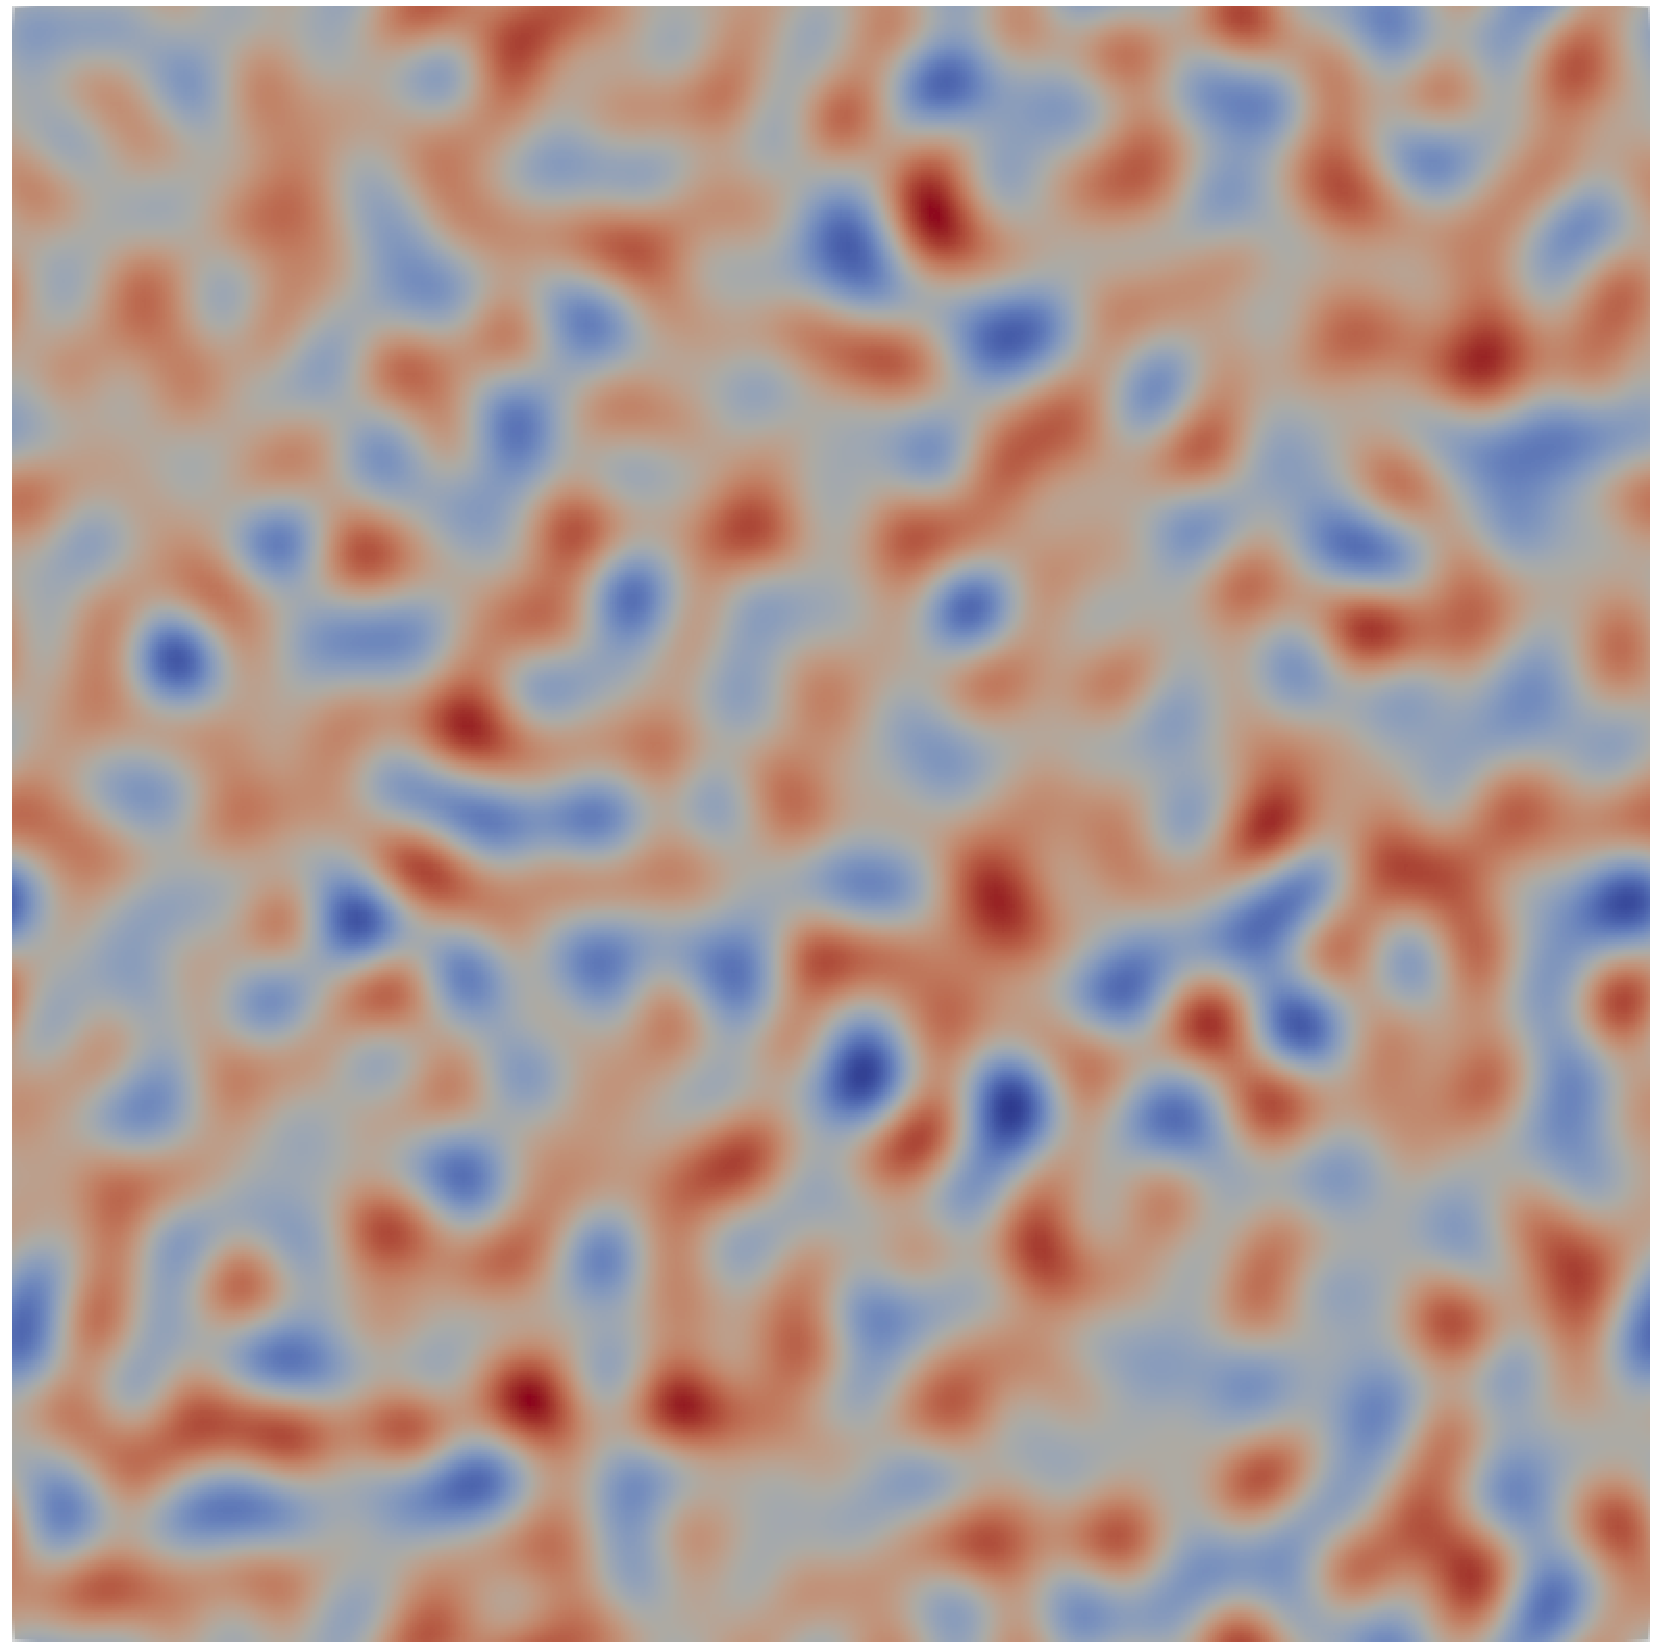
\includegraphics[width=0.95\textwidth]{Imagenes/Maxwell2D/Maxwell2D_sim/Imagenes/t_50}
        \caption{$t = 50$}
    \end{subfigure}
    \begin{subfigure}[t]{0.45\textwidth}
        \centering
        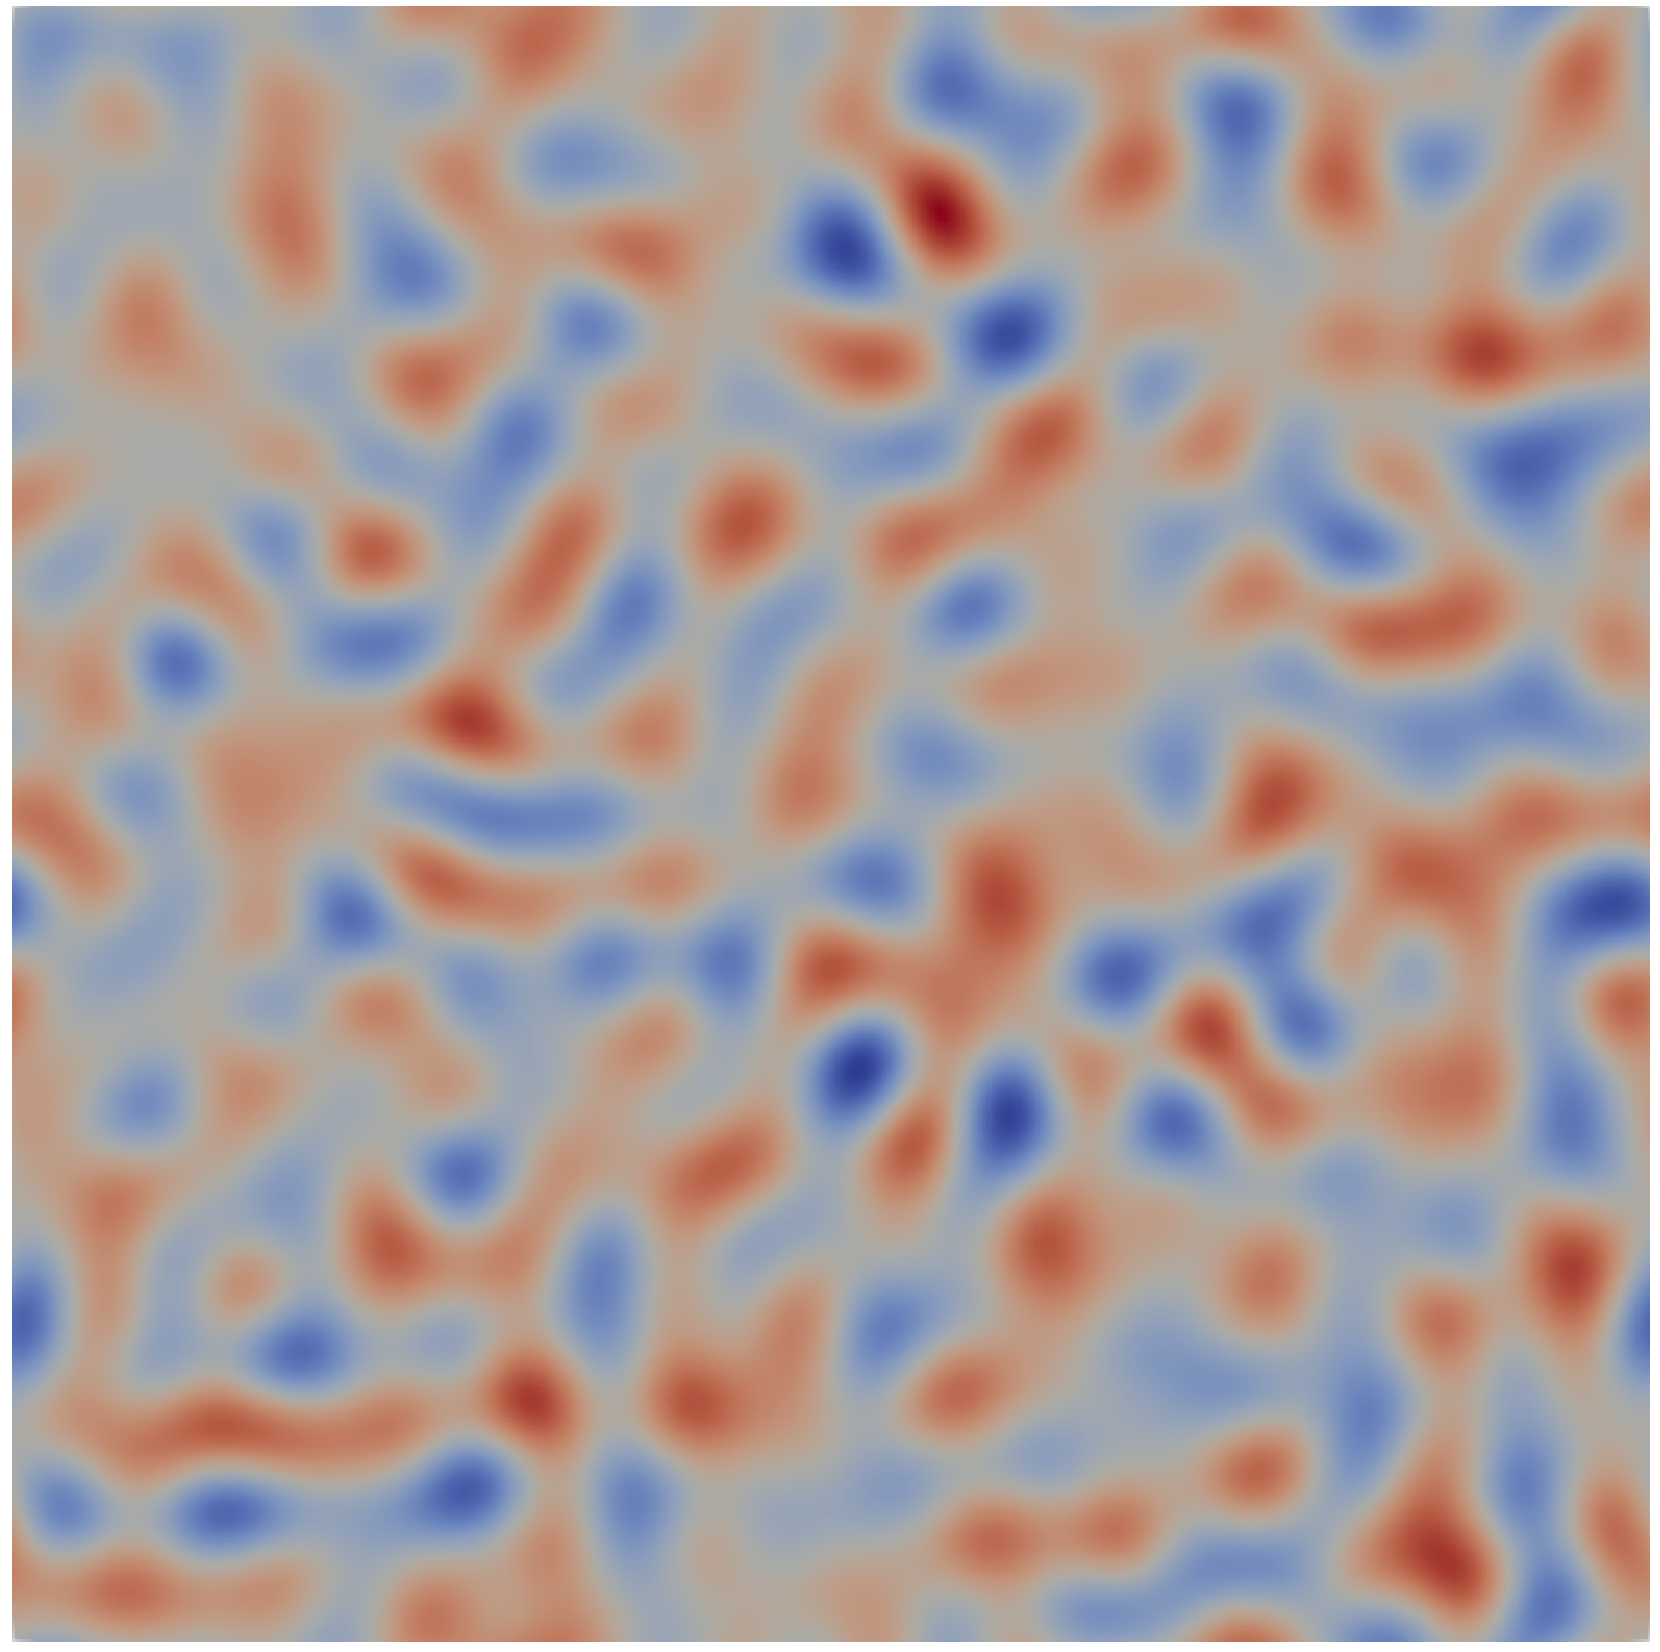
\includegraphics[width=0.95\textwidth]{Imagenes/Maxwell2D/Maxwell2D_sim/Imagenes/t_100}
        \caption{$t = 100$}
    \end{subfigure}    
    \begin{subfigure}[t]{0.45\textwidth}
        \centering
        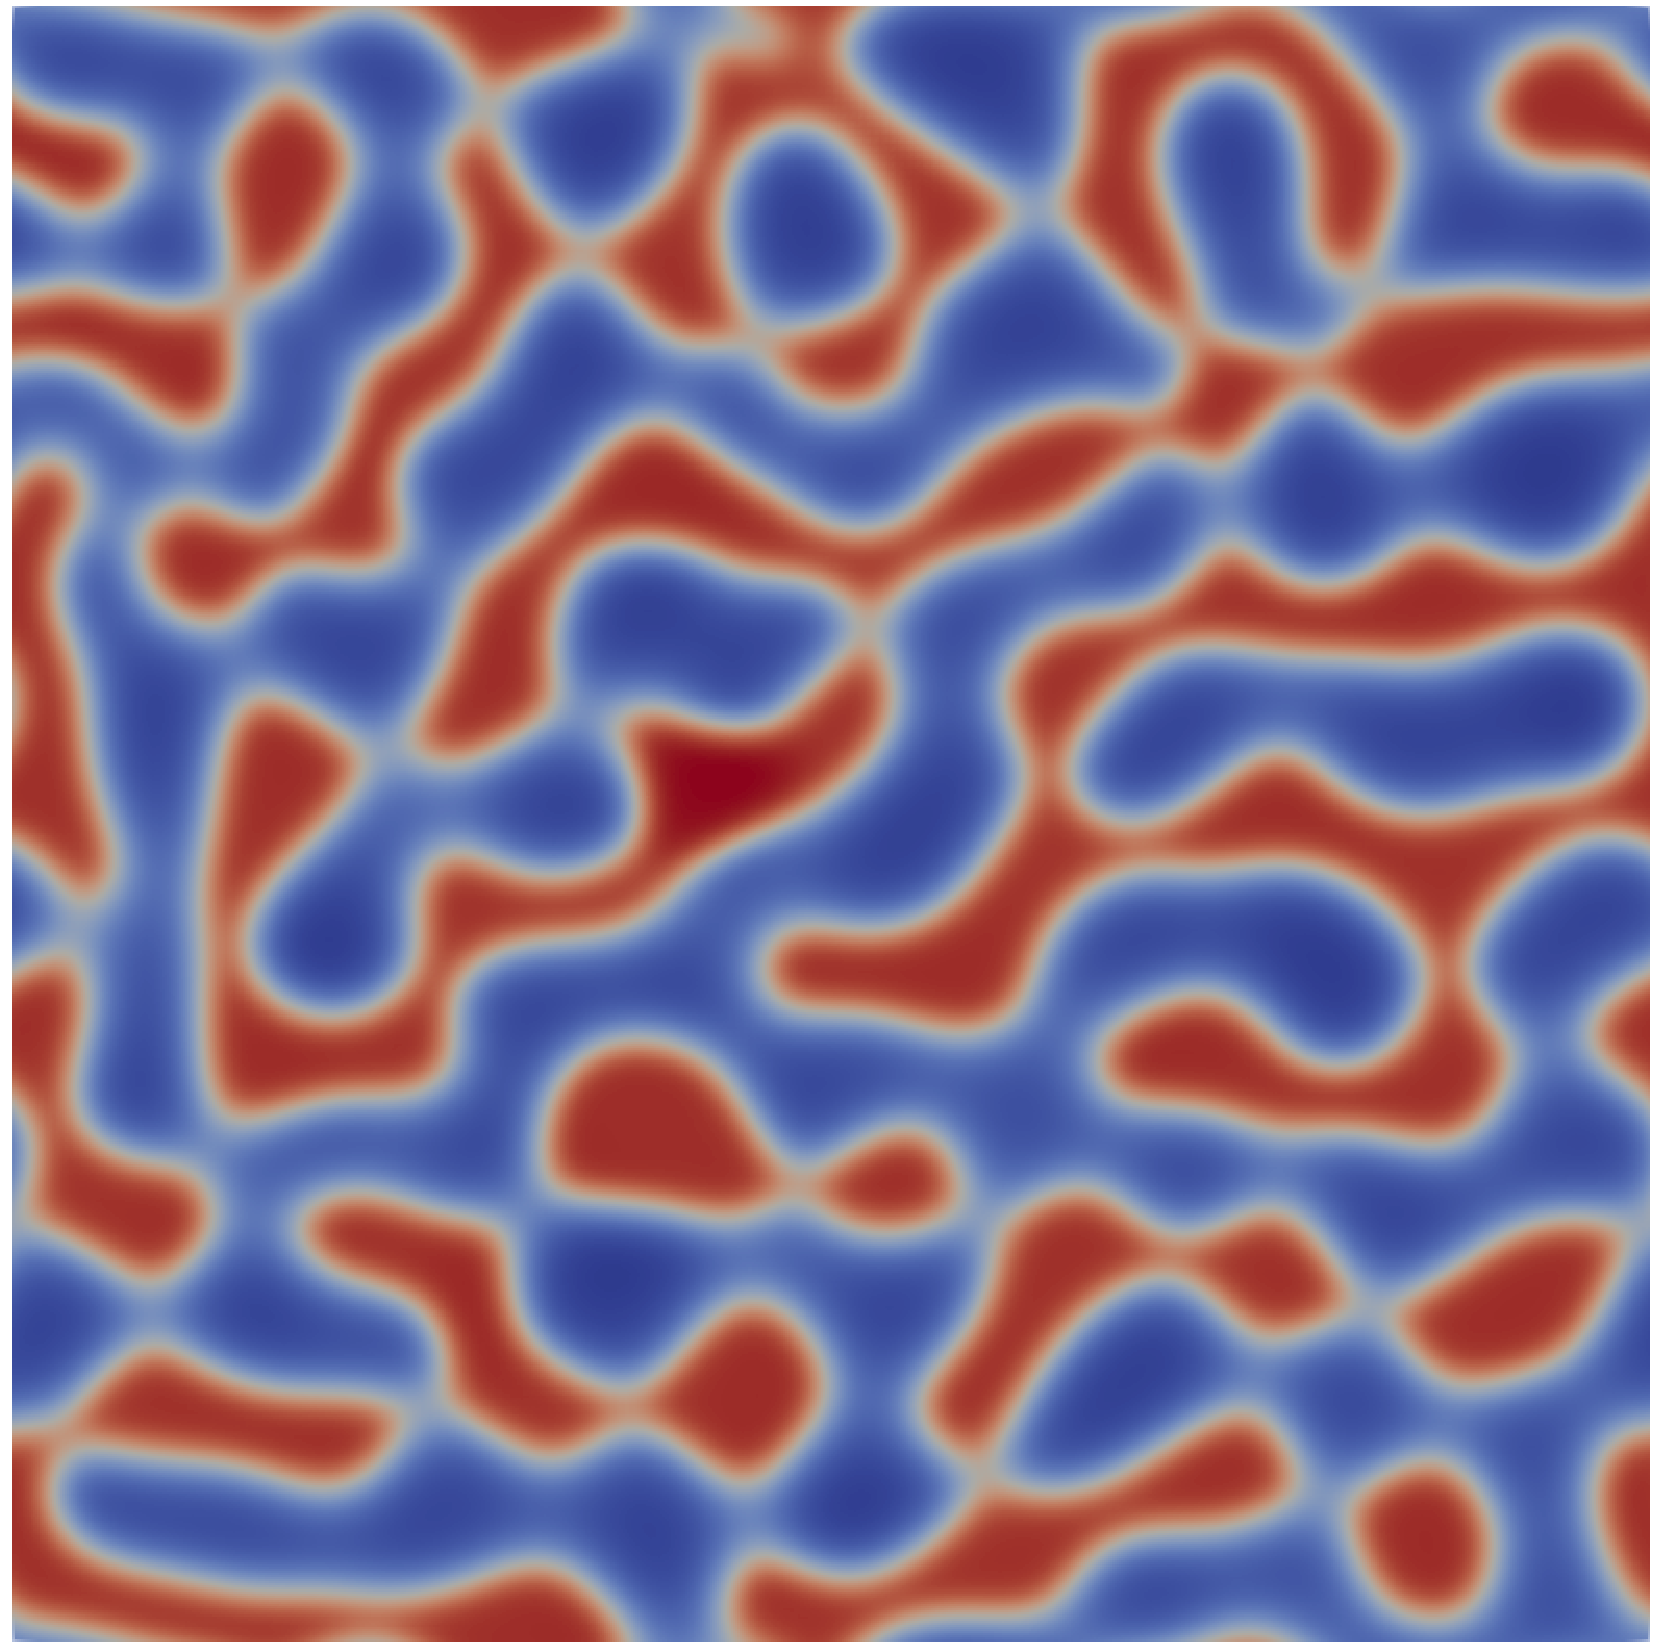
\includegraphics[width=0.95\textwidth]{Imagenes/Maxwell2D/Maxwell2D_sim/Imagenes/t_500}
        \caption{$t = 500$}
    \end{subfigure}    
    \begin{subfigure}[t]{0.45\textwidth}
        \centering
        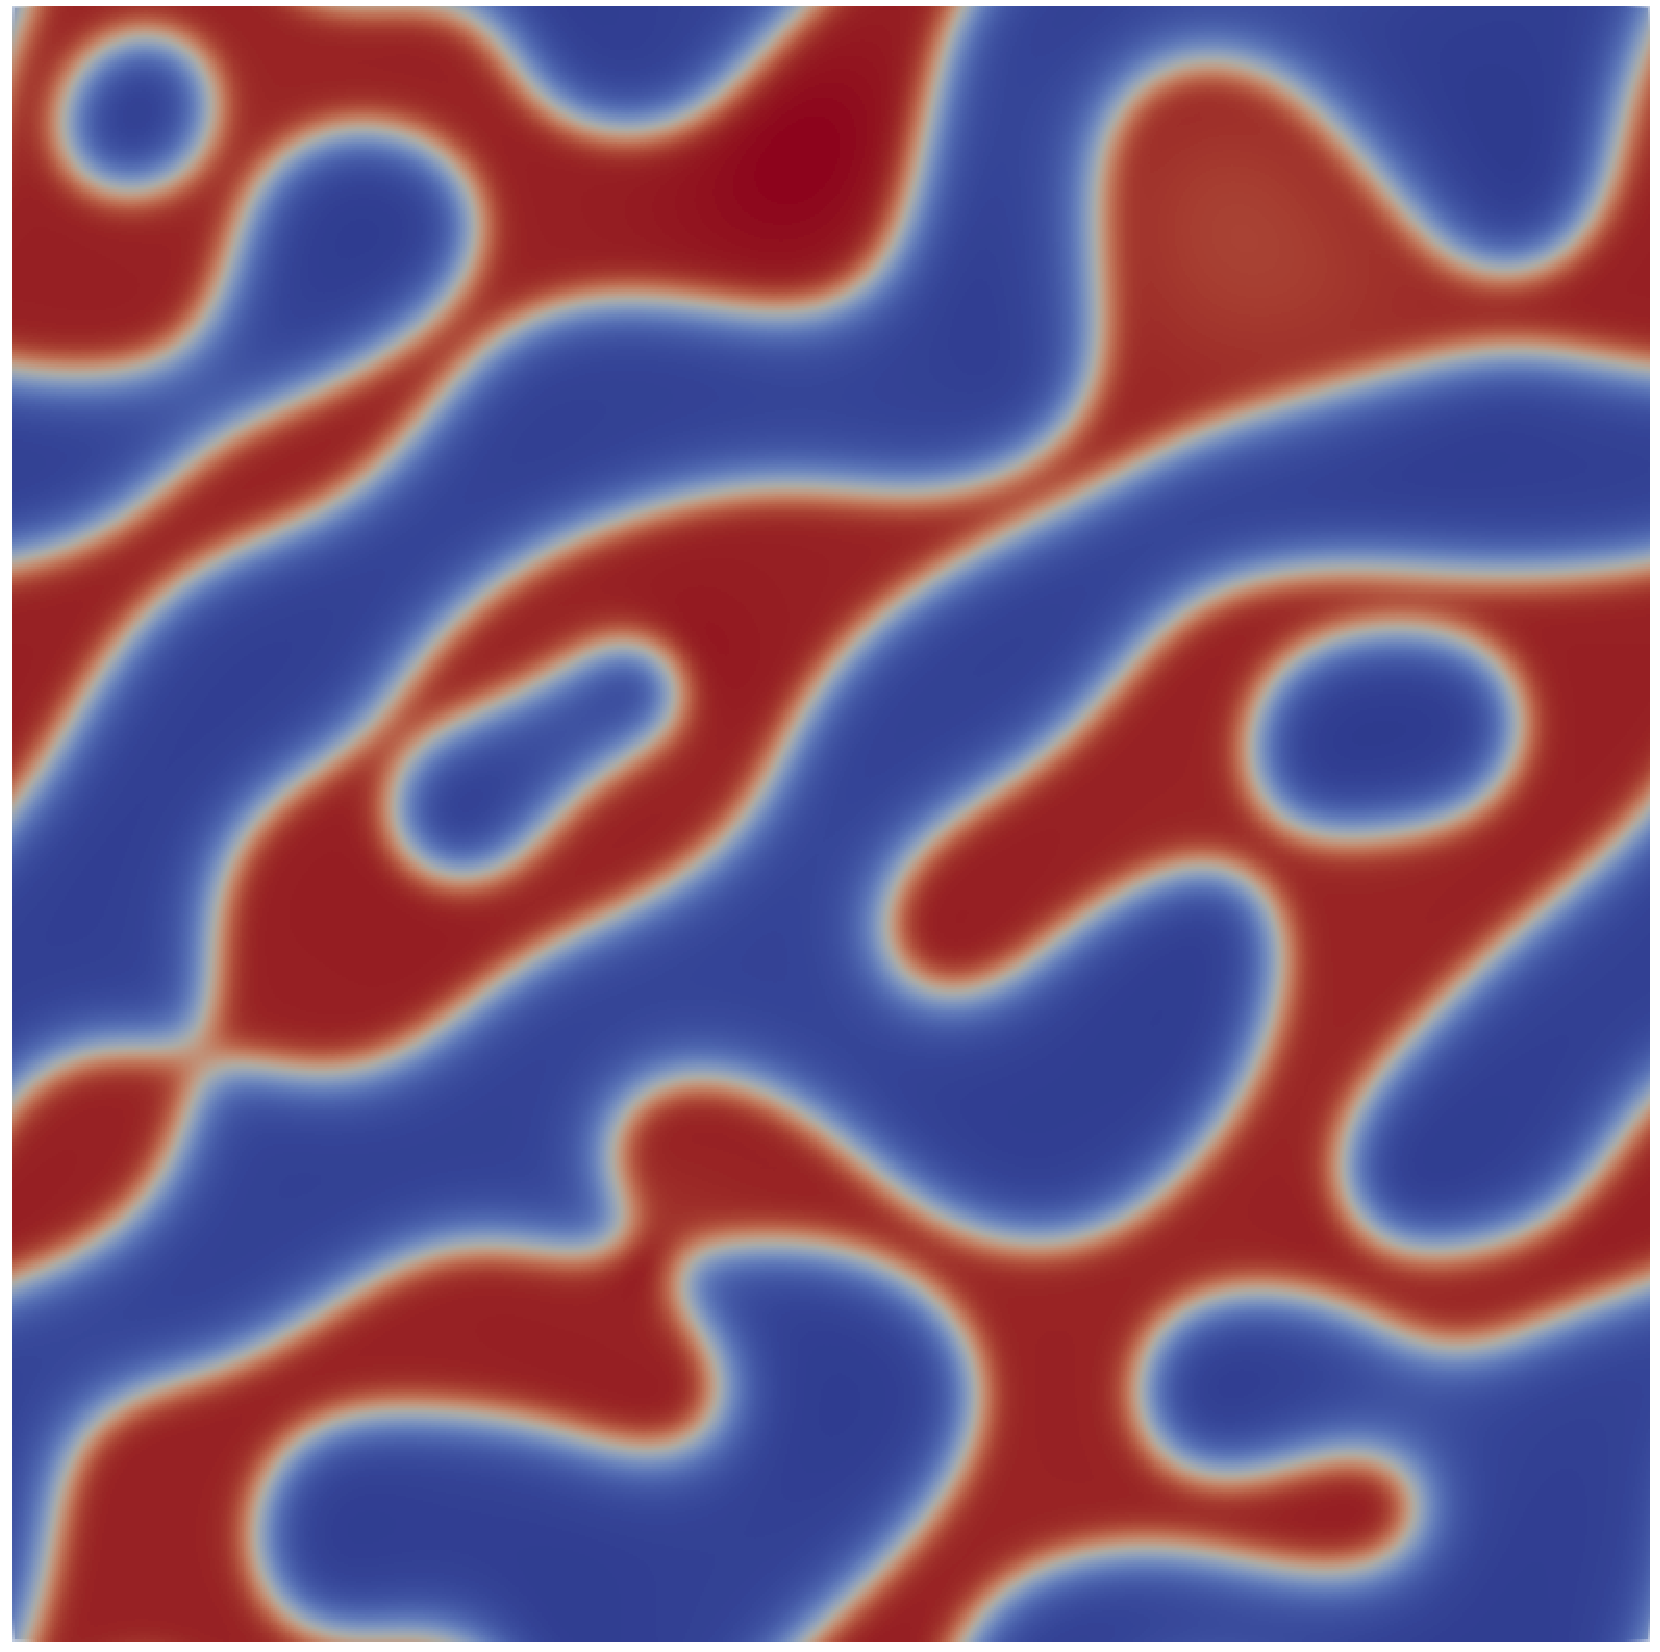
\includegraphics[width=0.95\textwidth]{Imagenes/Maxwell2D/Maxwell2D_sim/Imagenes/t_1000}
        \caption{$t = 1000$}
    \end{subfigure}
    \begin{subfigure}[t]{0.45\textwidth}
        \centering
        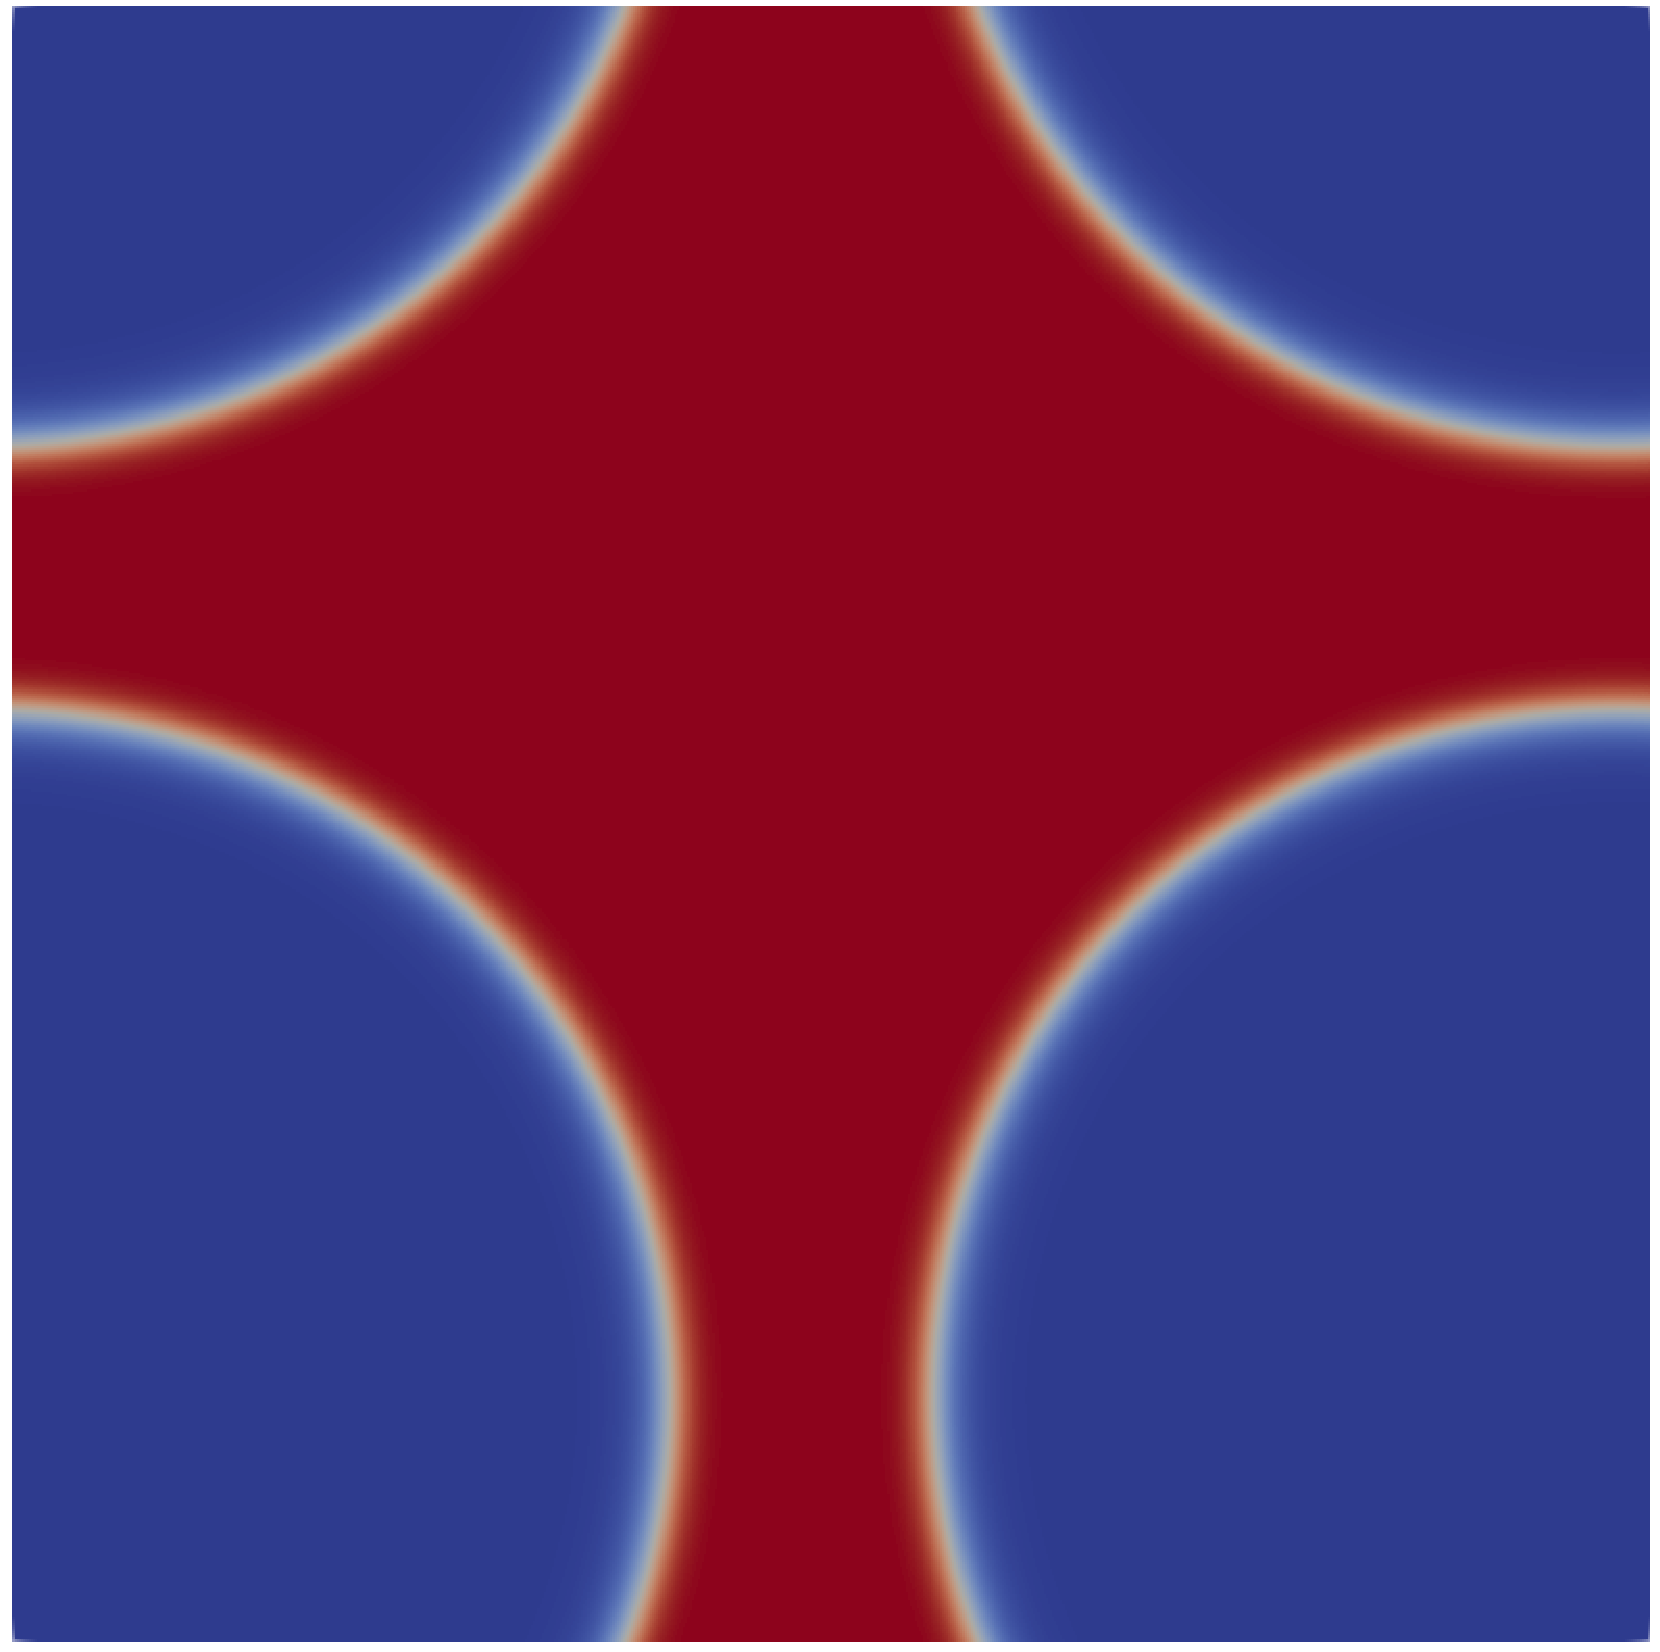
\includegraphics[width=0.95\textwidth]{Imagenes/Maxwell2D/Maxwell2D_sim/Imagenes/t_50000}
        \caption{$t = 50000$}
    \end{subfigure}        
    \caption{Evoluci\'on de una regi\'on tridimensional, peri\'odica, isot\'ermica y sin fuerzas externas, usada para verificar la regla de construcci\'on de Maxwell. La regi\'on mostrada corresponde a la fase de menor densidad.}
    \label{fig:maxwell_3d}
\end{figure}
\FloatBarrier
